\chapter{Energiberegning} \label{sec:energi}

Med henblik på at beregne rentabiliteten af de valgte energirenoveringstiltag, må den forventede besparelse kortlægges. Det gøres ved at betragte bygningens energiforbrug før og efter forbedringen. Hertil benyttes graddøgnsmetoden.

\section{Graddøgnsmetoden}

Graddage er et gammelt udtryk for et varmebehov angivet i enheden "grader gange dage". Det er således forskellen mellem en korrigeret indetemperatur og udetemperatur, ganget med en periode hvori temperaturforskellen har optrådt. Den korrigerede indetemperatur er lavere end rumtemperatur, idet der udnyttes et varmetilskud fra solindfald, personer og udstyr. Bygningens varmeanlæg skal således varme op til denne basistemperatur, som den kaldes. Graddagstal er baseret på basistemperaturen 17 $\decC$. Princippet er illustreret på figur \ref{fig:gdmetode}.

\begin{figure}[H]
	\centering
	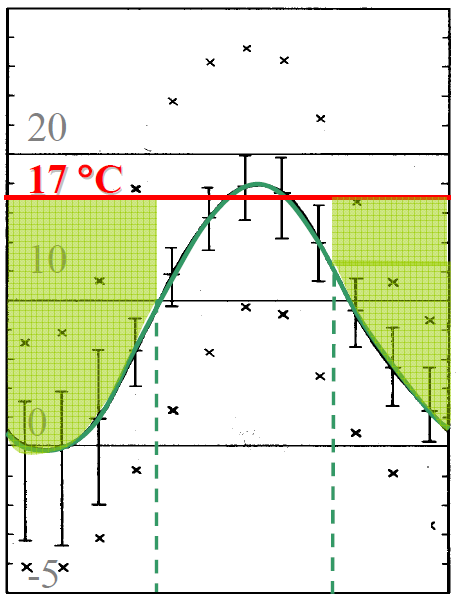
\includegraphics[width=0.55\textwidth]{billeder/graddage.png}
	\caption{Graddagene er illustreret som forskellen mellem basistemperaturen og udetemperaturen (i opvarmningssæsonen angivet med stiplede linjer) og er markeret med grønt.}
	\label{fig:gdmetode}
\end{figure}

Antallet af graddage årligt i Danmark er ca. 3.000. Når bygningsdelenes termiske egenskaber kendes, kan det forventede årlige energiforbrug, $E$, beregnes med ligning \eqref{eq:GD}. De anvendte forudsætninger kan findes i beskrivelsen af casehuset i appendiks \ref{sec:casehus}.

\begin{align}		
E = B_u \m 24 \m G			
\label{eq:GD} 
\end{align}

% \m er i preamble kodet til at gælde som \cdot (gangeprik) for at lette arbejdet

Hvor:
\begin{table}[H]
\begin{tabular}{l|l}
	$E$					& Det forventede energiforbrug [\si{Wh/\text{å}r}] \\
	$B_u$ 				& Bygningens specifikke varmetab ved transmission og ventilation [\si{W/K}] \\
	$24$ 				& Døgnets timer [\si{h/d\text{ø}gn}] \\
	$G$					& Graddage [\si{K d\text{ø}gn/\text{å}r}]
\end{tabular}
\end{table}

Bygningens specifikke varmetab består af bidrag fra transmissionstab og ventilationstab.\fxnote{Skriv færdigt i morgen}

